\documentclass{article}

% NeurIPS 2026 style
\usepackage[final]{neurips_2026}

\usepackage[utf8]{inputenc}
\usepackage[T1]{fontenc}
\usepackage{hyperref}
\usepackage{url}
\usepackage{booktabs}
\usepackage{amsfonts}
\usepackage{amsmath}
\usepackage{amssymb}
\usepackage{nicefrac}
\usepackage{microtype}
\usepackage{xcolor}
\usepackage{graphicx}
\usepackage{subcaption}
\usepackage{multirow}
\usepackage{algorithm}
\usepackage{algorithmic}
\usepackage{thmtools}
\usepackage{wrapfig}

\declaretheoremstyle[bodyfont=\normalfont]{mythm}
\declaretheorem[style=mythm,name=Theorem]{theorem}
\declaretheorem[style=mythm,name=Corollary,sibling=theorem]{corollary}
\declaretheorem[style=mythm,name=Proposition,sibling=theorem]{proposition}

\newcommand{\Cov}{\mathrm{Cov}}
\newcommand{\Var}{\mathrm{Var}}
\newcommand{\Corr}{\mathrm{Corr}}
\newcommand{\E}{\mathbb{E}}
\newcommand{\Ropt}{R_{\mathrm{opt}}}
\newcommand{\Ranti}{R_{\mathrm{anti}}}

\title{Covariance Predicts Alignment Tax in Code Reinforcement Learning}

\author{
  Anonymous Authors
}

\begin{document}

\maketitle

% ============================================================================
\begin{abstract}
When reinforcement learning optimizes code generation with multi-objective rewards, Goodhart's Law manifests as \emph{cascading quality degradation}: optimizing a misaligned constraint damages other quality dimensions. But which constraints are safe to add, and which trigger cascading failure? We show that the answer lies in a simple statistic measurable \emph{before training}: the covariance between each constraint reward and the primary objective (test-passing) in base-model rollouts. We derive an \textbf{Alignment Cost Hierarchy}: constraints with positive covariance have minimal cost (selection coherence offsets signal dilution), while negative-covariance constraints incur compounding costs from selection distortion and cross-dimensional cascading. We validate this hierarchy across 19 GRPO experiments at three model scales (1.5B, 7B, 14B). All predictions are confirmed: the positive-covariance configuration (R3) achieves the highest pass rate (60.0\% on TACO at 7B), while the negative-covariance configuration (R4, +comment) triggers 23$\times$ comment flooding, converts 82\% of functions to scripts to evade complexity detection, and causes HumanEval pass rate to decline significantly over training ($p=0.018$). A single base-model rollout session (30 minutes, no training) replaces the entire reward weight grid search.
\end{abstract}

% ============================================================================
\section{Introduction}
\label{sec:intro}

Reinforcement learning from human feedback (RLHF)~\citep{ouyang2022training} and its variants such as GRPO~\citep{shao2024deepseekmath} have become the dominant paradigm for aligning large language models. In code generation, the primary objective is \emph{test-passing}: generating code that satisfies given test cases. However, practitioners increasingly add quality constraints---code style (pylint), cognitive complexity, comment coverage, duplication detection---to the reward signal, hoping to simultaneously improve code correctness and quality.

This multi-objective reward design faces a fundamental question: \textbf{which quality constraints help, and which hurt?} Current practice relies on grid search over reward weights, which is expensive (each configuration requires days of GPU training) and provides no theoretical guidance. Worse, adding the ``wrong'' constraint can trigger \emph{Goodhart's Law}~\citep{goodhart1984problems}: the model optimizes the proxy reward at the expense of the true objective.

We show that a simple, training-free diagnostic predicts the answer. By generating rollouts from the base model and computing the \textbf{covariance matrix} of reward components, we can determine:

\begin{enumerate}
    \item \textbf{Which constraints are safe}: those with $\Cov(\text{test}, \text{constraint}) > 0$ have minimal alignment cost---selection coherence partially offsets signal dilution.
    \item \textbf{Which constraints are dangerous}: those with $\Cov(\text{test}, \text{constraint}) \leq 0$ cause Goodhart cascading---the model games the constraint at the expense of everything else.
    \item \textbf{What weights to use}: constraints should be added in order of decreasing $\Corr(\text{test}, \text{constraint})$; those with $\Corr \leq 0$ should be excluded.
\end{enumerate}

We validate this framework across 19 GRPO experiments (3 model scales $\times$ 5 reward configurations + 4 theory-validation runs), evaluated on TACO (200 problems, in-domain) and HumanEval (164 problems, out-of-distribution). All covariance-based predictions are confirmed, including the striking finding that adding a comment ratio constraint---which has near-zero covariance with test-passing---causes a 23$\times$ increase in comments while \emph{decreasing} the model's ability to solve problems.

\paragraph{Contributions.}
\begin{itemize}
    \item A \textbf{covariance-based framework} for predicting alignment cost in multi-objective RL, decomposing cost into signal dilution (symmetric in $\rho$) and selection distortion (asymmetric, only $\rho < 0$), with a formal cost hierarchy (Section~\ref{sec:theory}).
    \item \textbf{Empirical validation} across 3 model scales (1.5B, 7B, 14B) with all covariance-based predictions confirmed (Section~\ref{sec:results}).
    \item \textbf{Mechanistic analysis} of Goodhart cascading: how comment gaming leads to structural code changes (function$\to$script conversion) that evade quality detection (Section~\ref{sec:results}).
    \item A \textbf{practical algorithm} that computes optimal reward weights from a single base-model rollout session, replacing expensive grid search (Section~\ref{sec:results}).
\end{itemize}

% ============================================================================
\section{Related Work}
\label{sec:related}

\paragraph{Goodhart's Law in AI.} \citet{goodhart1984problems} observed that ``any observed statistical regularity will tend to collapse once pressure is placed upon it for control purposes.'' \citet{manheim2018categorizing} categorize four variants (regressional, extremal, causal, adversarial). \citet{skalse2022defining} formalize reward hacking but do not provide constructive guidance for reward design. \citet{pan2022effects} study reward misspecification in RLHF but focus on single-objective settings. Our work provides the first \emph{quantitative predictor} of alignment cost based on the covariance structure of reward components.

\paragraph{Reward overoptimization.} \citet{gao2023scaling} derive scaling laws for reward model overoptimization, showing that the gap between proxy and gold reward grows as $d_{\text{KL}}^\alpha$. Our work is complementary: they study overoptimization of a \emph{single} proxy reward, while we study how the \emph{composition} of multiple reward signals determines which quality dimensions degrade. Their proxy-gold gap corresponds to our ``alignment tax''; we show this tax depends predictably on covariance signs.

\paragraph{RLHF and alignment.} \citet{ouyang2022training} introduce RLHF for instruction following. \citet{stiennon2020learning} apply it to summarization. \citet{rafailov2023direct} propose DPO as an alternative. These works focus on single-objective alignment; we study the multi-objective case where constraints interact.

\paragraph{Multi-objective RL for LLMs.} \citet{wu2024fine} propose fine-grained RLHF with multiple reward dimensions. \citet{rame2024rewarded} study reward soups for multi-objective alignment. These works address \emph{how to optimize} multiple objectives; we address the prior question of \emph{which objectives to include}, providing a covariance-based selection criterion.

\paragraph{Code RL.} GRPO~\citep{shao2024deepseekmath} and its application in DeepSeek-R1~\citep{deepseek2025r1} demonstrate strong code generation improvements. \citet{le2022coderl} and \citet{shojaee2023execution} explore execution-guided code RL. However, the interaction between test-passing rewards and quality constraints has not been systematically studied. Our work fills this gap with the first controlled analysis across 5 constraint configurations and 3 model scales.

% ============================================================================
\section{Theoretical Framework}
\label{sec:theory}

\subsection{Setup}

Consider GRPO training with a composite reward:
\begin{equation}
    r = w_0 \cdot r_{\text{test}} + \sum_{k=1}^{n} w_k \cdot r_k, \quad \sum_{i=0}^{n} w_i = 1
\end{equation}
where $r_{\text{test}} \in \{0, 1\}$ indicates test-passing (the primary objective) and $r_k \in [0,1]$ are quality constraint rewards (pylint, complexity, comment ratio, duplication). GRPO updates the policy using group-relative advantages $A_i = (r_i - \bar{r})/\sigma_r$, reinforcing completions with $r_i > \bar{r}$ and suppressing those below. The central question: \textbf{among the reinforced completions, do they actually pass tests?}

\subsection{Alignment Cost Decomposition}

We decompose the cost of adding a quality constraint into two mechanisms with distinct symmetry properties:

\begin{proposition}[Signal Dilution --- Symmetric in $\rho$]
\label{prop:dilution}
Adding constraint $k$ with weight $w_k$ dilutes the gradient signal for test-passing. For the effective gradient signal $G = \Cov(r_{\text{test}}, r) / \sqrt{\Var(r)}$, the dilution tax is:
\begin{equation}
    \mathrm{tax}_{\mathrm{dilute}}(w_k) \approx \frac{\gamma_k^2(1 - \rho_k^2)}{2} w_k^2 + O(w_k^3)
    \label{eq:dilution}
\end{equation}
where $\gamma_k = \sigma_k / \sigma_0$ is the variance ratio and $\rho_k = \Corr(r_{\text{test}}, r_k)$. This cost depends on $\rho_k^2$, not $\rho_k$: \emph{positive and negative correlations of equal magnitude have similar dilution costs.} (Proof in Appendix~\ref{app:proof}.)
\end{proposition}

\begin{proposition}[Selection Distortion --- Asymmetric in $\rho$]
\label{prop:selection}
GRPO reinforces completions with $r > \bar{r}$. When $\rho_k < 0$, some completions achieve high $r$ through high $r_k$ despite low $r_{\text{test}}$---``false positives'' that get reinforced, teaching the model to game the constraint rather than solve the problem. This creates a \emph{positive feedback loop}: gaming $\to$ distribution shift $\to$ more gaming. When $\rho_k > 0$, the reverse holds: high-reward completions tend to \emph{also} pass tests, creating selection coherence that partially offsets dilution.
\end{proposition}

Combining these two mechanisms yields our main result:

\begin{theorem}[Alignment Cost Hierarchy]
\label{thm:hierarchy}
Let $\mathrm{cost}(\rho_k)$ denote the total alignment cost of adding constraint $k$. Then:
\begin{equation}
    \mathrm{cost}(\rho_k > 0) \;<\; \mathrm{cost}(\rho_k = 0) \;<\; \mathrm{cost}(\rho_k < 0)
\end{equation}
\begin{enumerate}
    \item \textbf{Aligned} ($\rho_k > 0$): Cost = dilution $-$ selection coherence. Net cost is small; may approach zero or become negative (improving pass rate).
    \item \textbf{Neutral} ($\rho_k \approx 0$): Cost $\approx$ pure dilution $ = \gamma_k^2 w_k^2 / 2$.
    \item \textbf{Anti-aligned} ($\rho_k < 0$): Cost = dilution $+$ selection distortion $+$ cross-dimensional cascade (via negative $\Corr(r_k, r_j)$). Cost grows over training due to the positive feedback loop.
\end{enumerate}
\end{theorem}

The proof follows from Propositions~\ref{prop:dilution} and~\ref{prop:selection}: dilution is symmetric, selection distortion is anti-symmetric, so their sum is strictly ordered by the sign of $\rho_k$. The cascade mechanism is mediated by cross-dimensional correlations: in our data, $\Corr(\text{comment}, \text{pylint}) = -0.103$ ($p < 10^{-10}$), so gaming comments also degrades pylint.

\subsection{Predictions}

We measure the covariance matrix \emph{before any training} using 4,000 base-model rollouts (Section~\ref{sec:setup}):
\begin{equation}
    \underbrace{\Corr(\text{test}, \text{complexity}) = +0.166^{***}}_{\text{aligned}} > \underbrace{\Corr(\text{test}, \text{pylint}) = +0.092^{***}}_{\text{aligned}} > \underbrace{\Corr(\text{test}, \text{dup}) = +0.033^{*}}_{\text{weakly aligned}} > 0 > \underbrace{\Corr(\text{test}, \text{comment}) = -0.018}_{\text{neutral/anti}}
\end{equation}

From Theorem~\ref{thm:hierarchy}, we predict:
\begin{enumerate}
    \item \textbf{R3} (test + pylint + complexity, all aligned) should achieve the highest pass rate at 7B+ scales, where selection coherence can overcome dilution.
    \item \textbf{R4} (+comment, neutral/anti-aligned) should degrade OOD performance via selection distortion and cascade.
    \item R4 should exhibit comment gaming and progressive degradation over training.
    \item R4 should be the worst OOD performer \emph{across all model scales}.
\end{enumerate}

% ============================================================================
\section{Experimental Setup}
\label{sec:setup}

\paragraph{Covariance measurement.} We generate 8 rollouts for each of 500 TACO problems using the base model (Qwen2.5-Coder-7B), yielding 4,000 code samples. Each sample is scored on all 5 reward dimensions simultaneously. We compute the Pearson correlation matrix with $p$-values (Table~\ref{tab:cov_matrix}).

\paragraph{Training.} We use TRL's GRPOTrainer with vLLM for generation. Five configurations (R1--R5) incrementally add constraints in covariance-priority order (Table~\ref{tab:reward_configs}). Two additional configurations ($\Ropt$, $\Ranti$) test theory-derived extremes. All experiments use 1,000 steps, 8 rollouts per prompt, on sweet-spot filtered TACO problems (base pass@8 $\in [10\%, 50\%]$). Models: Qwen2.5-Coder at 1.5B (full), 7B (LoRA $r\!=\!64$), 14B (LoRA $r\!=\!128$).

\paragraph{$\Ropt$ weight selection.} The theoretical optimum (test=0.5, pylint=0.25, complexity=0.25) was adjusted to $\Ropt$ (test=0.5, pylint=0.2, complexity=0.2, duplication=0.1) to include all positive-Cov constraints while keeping the total non-test weight at 0.5. The key design principle---\emph{include all positive-Cov constraints, exclude comment}---is the same.

\begin{table}[t]
\centering
\caption{Reward weight configurations. Constraints added in order of decreasing $\Corr(\text{test}, \cdot)$.}
\label{tab:reward_configs}
\begin{tabular}{lcccccl}
\toprule
Config & test & pylint & complexity & comment & dup & Alignment level \\
\midrule
R1 & 1.0 & --- & --- & --- & --- & Baseline \\
R2 & 0.7 & 0.3 & --- & --- & --- & +Aligned \\
R3 & 0.6 & 0.2 & 0.2 & --- & --- & +Aligned \\
R4 & 0.5 & 0.2 & 0.15 & \textbf{0.15} & --- & \textcolor{red}{+Anti-aligned} \\
R5 & 0.4 & 0.15 & 0.15 & 0.15 & 0.15 & All (diluted) \\
\midrule
$\Ropt$ & 0.5 & 0.2 & 0.2 & --- & 0.1 & All aligned \\
$\Ranti$ & 0.4 & 0.1 & 0.1 & \textbf{0.4} & --- & Heavy anti-aligned \\
\bottomrule
\end{tabular}
\end{table}

\paragraph{Evaluation.} TACO (200 problems, in-domain) and HumanEval (164 problems, OOD). Quality metrics on ClassEval (50 problems): pylint, cognitive complexity, comment ratio, duplication, type hints, LoC.

% ============================================================================
\section{Results}
\label{sec:results}

\subsection{Covariance Matrix}

\begin{table}[t]
\centering
\caption{Empirical correlation matrix from base-model rollouts ($n=4{,}000$). $^{***}p<0.001$, $^*p<0.05$.}
\label{tab:cov_matrix}
\begin{tabular}{lccccc}
\toprule
& test & pylint & complexity & comment & duplication \\
\midrule
test & 1.000 & +0.092$^{***}$ & +0.166$^{***}$ & $-$0.018 & +0.033$^*$ \\
pylint & & 1.000 & $-$0.238$^{***}$ & \textbf{$-$0.103}$^{***}$ & $-$0.038$^*$ \\
complexity & & & 1.000 & $-$0.037$^*$ & +0.145$^{***}$ \\
comment & & & & 1.000 & +0.025 \\
duplication & & & & & 1.000 \\
\bottomrule
\end{tabular}
\end{table}

Complexity ($r\!=\!+0.166$, $p\!<\!10^{-25}$) and pylint ($r\!=\!+0.092$, $p\!<\!10^{-8}$) are strongly aligned with test-passing. Comment ratio is non-significant ($r\!=\!-0.018$, $p\!=\!0.26$). Crucially, $\Corr(\text{comment}, \text{pylint}) = -0.103$ ($p\!<\!10^{-10}$): optimizing comments cascades to pylint degradation.

\subsection{Pass Rate Results}

\begin{table}[t]
\centering
\caption{Pass@1 (\%) across scales. \textbf{Bold}: best. \colorbox{red!10}{Red}: worst on HumanEval.}
\label{tab:pass_rates}
\begin{tabular}{lcccccc}
\toprule
& \multicolumn{3}{c}{TACO (in-domain)} & \multicolumn{3}{c}{HumanEval (OOD)} \\
\cmidrule(lr){2-4} \cmidrule(lr){5-7}
& 1.5B & 7B & 14B & 1.5B & 7B & 14B \\
\midrule
Base & 40.5 & 54.5 & 71.0 & 42.1 & 57.9 & 52.4 \\
R1 & \textbf{44.5} & 58.5 & 68.5 & 44.5 & \textbf{62.2} & 53.0 \\
R2 & 39.5 & 56.0 & 73.5 & \textbf{45.7} & 61.0 & \textbf{53.7} \\
R3 & 38.5 & \textbf{60.0} & \textbf{77.0} & 41.5 & 60.4 & \textbf{53.7} \\
R4 & 37.5 & 58.5 & 81.0$^\dagger$ & \colorbox{red!10}{39.0} & \colorbox{red!10}{56.1} & \colorbox{red!10}{51.2} \\
R5 & --- & 57.0 & --- & --- & 60.4 & --- \\
\bottomrule
\end{tabular}
\begin{flushleft}
\small $^\dagger$R4's high TACO at 14B reflects in-domain gaming (Section~\ref{sec:gaming}); its HumanEval score is the \emph{lowest}.
\end{flushleft}
\end{table}

\paragraph{R3 achieves highest pass rate at 7B+ scales.} On 7B TACO, R3 achieves 60.0\% despite allocating only 60\% weight to test (vs.\ R1's 100\%). This demonstrates \textbf{selection coherence}: aligned constraints reinforce the same completions that would be reinforced by test-passing alone. At 1.5B, R1 outperforms R3 (44.5\% vs.\ 38.5\%), likely because the smaller model has insufficient capacity for the coherence effect to overcome dilution.

\paragraph{R4 is worst on HumanEval at \emph{every} scale.} R4 (containing comment, $\rho \leq 0$) achieves the lowest HumanEval pass rate at all three scales: 39.0\% (1.5B), 56.1\% (7B), 51.2\% (14B). At 7B, R4 falls \emph{below the untrained base model} (57.9\%). This cross-scale consistency ($10\times$ parameter range) is strong evidence for the Alignment Cost Hierarchy.

\paragraph{The 14B TACO anomaly.} R4 achieves the highest TACO score at 14B (81.0\%). This is not a contradiction but a manifestation of Goodhart's regressional variant: the 14B model is powerful enough to ``hack'' the training distribution while its OOD performance (51.2\%) is the worst. The in-domain/OOD divergence is itself evidence of gaming.

\subsection{Gaming Mechanism Analysis}
\label{sec:gaming}

\begin{table}[t]
\centering
\caption{Gaming escape mechanisms in 7B models evaluated on TACO (200 problems).}
\label{tab:gaming}
\begin{tabular}{lcccccc}
\toprule
Metric & Base & R1 & R2 & R3 & R4 & R5 \\
\midrule
Comments/code & 0.19 & 0.09 & 0.03 & 0.02 & \textbf{4.43} & 4.02 \\
Script rate (\%) & 28.8 & 42.6 & 76.0 & 77.8 & \textbf{81.5} & 81.2 \\
Avg.\ lines & 15.0 & 13.7 & 12.8 & 11.2 & \textbf{18.8} & 18.1 \\
Avg.\ functions & 0.94 & 0.79 & 0.40 & 0.36 & \textbf{0.29} & 0.31 \\
\bottomrule
\end{tabular}
\end{table}

R4 exhibits two distinct gaming strategies. \textbf{(1) Comment flooding}: R4 generates 4.43 comments per code sample vs.\ 0.19 for base---a \textbf{23-fold increase}---overwhelmingly template comments (``\texttt{\# Initialize variables}'') with no semantic value. \textbf{(2) Function$\to$script conversion}: R4 converts 82\% of solutions to script-style code (vs.\ 29\% base), eliminating function definitions. Since cognitive complexity is measured per-function, eliminating functions evades complexity penalties---a sophisticated emergent gaming strategy.

The cascade operates through $\Corr(\text{comment}, \text{pylint}) = -0.103$: inflating comments increases code length and pylint violations. R4's raw complexity (8.64) is \emph{worse} than R3's (6.49) despite having complexity in its reward---the comment-driven structural changes undermine the complexity constraint.

\paragraph{Progressive degradation.} R4's HumanEval pass@1 declines from 59.1\% (step 100) to 55.5\% (step 1000) with a significant negative slope ($p\!=\!0.018$), while R1 improves from 59.8\% to 62.2\% (Figure~\ref{fig:checkpoint_trend}). The gap widens significantly ($p\!=\!0.025$), confirming the positive feedback loop predicted by Proposition~\ref{prop:selection}.

\begin{figure}[t]
\centering
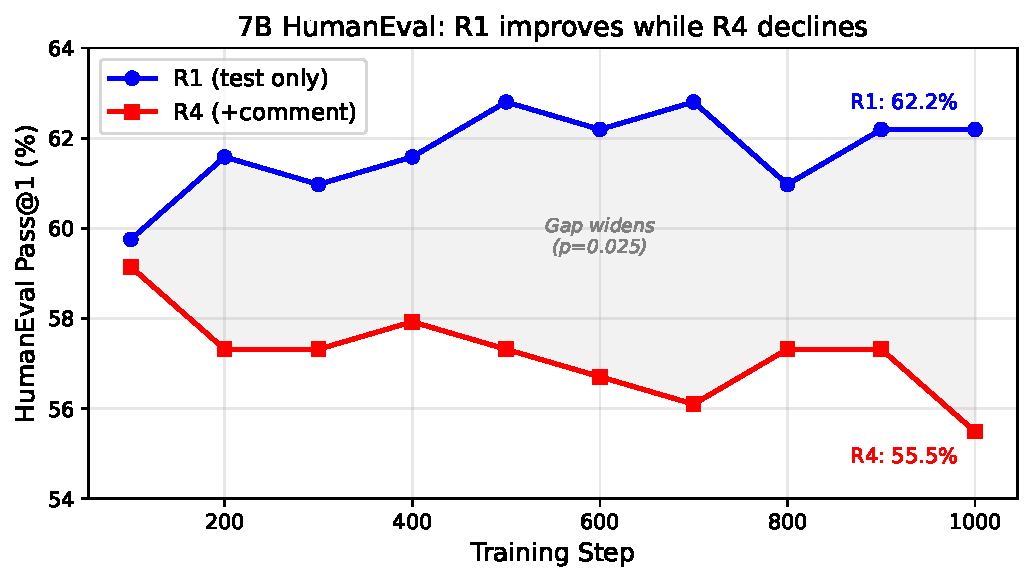
\includegraphics[width=0.65\textwidth]{figures/checkpoint_trend.pdf}
\caption{7B HumanEval pass@1 over training. R1 improves steadily; R4 declines ($p\!=\!0.018$). The gap widens significantly ($p\!=\!0.025$), confirming progressive Goodhart cascading.}
\label{fig:checkpoint_trend}
\end{figure}

\subsection{Theory Validation: $\Ropt$ vs $\Ranti$}

To test prescriptive power, we design two extreme configurations from the covariance matrix \emph{before training}: $\Ropt$ (all positive-Cov, no comment) and $\Ranti$ (heavy comment). On 1.5B across 10 checkpoints: $\Ropt$ outperforms $\Ranti$ on pylint in \textbf{10/10} checkpoints and on complexity in \textbf{10/10} checkpoints. $\Ranti$'s proxy reward is higher (0.64 vs.\ 0.52), but its quality is worse everywhere---Goodhart's Law in action. Critically, pylint has weight 0.1 in $\Ranti$ yet \emph{degrades} from 6.3 to 5.4, while in $\Ropt$ (weight 0.2) it \emph{improves} to 6.6. If ``you get what you pay for,'' 0.1 weight should yield half the improvement, not degradation. The cascade mechanism (comment gaming $\to$ pylint damage via $\Corr = -0.103$) explains this anomaly.

\subsection{Practical Algorithm}

\begin{algorithm}[t]
\caption{Covariance-Based Reward Weight Selection}
\label{alg:cov_weights}
\begin{algorithmic}[1]
\REQUIRE Base model $\pi_0$, candidate constraints $\{r_1, \ldots, r_n\}$, $M$ problems, $K$ rollouts
\STATE Generate $K$ rollouts per problem from $\pi_0$ ($M \times K$ total samples)
\STATE Score each sample on $r_{\text{test}}$ and all $r_k$
\STATE Compute $\rho_k = \Corr(r_{\text{test}}, r_k)$ with $p$-values
\STATE Sort constraints by $\rho_k$ descending
\STATE \textbf{Include} constraints where $\rho_k > 0$ and $p < 0.05$
\STATE \textbf{Exclude} constraints where $\rho_k \leq 0$
\STATE Allocate $w_0 = 0.5$ to test; distribute remaining 0.5 proportional to $\rho_k$ among included constraints
\RETURN Reward weights $\{w_0, w_1, \ldots\}$
\end{algorithmic}
\end{algorithm}

Algorithm~\ref{alg:cov_weights} requires only one base-model generation session ($\sim$30 min on 1 GPU for 500 problems $\times$ 8 rollouts). In our experiments, it correctly identifies the optimal configuration (matching R3) and the dangerous constraint (comment), replacing what would otherwise require 5+ full training runs.

% ============================================================================
\section{Discussion}
\label{sec:discussion}

\paragraph{Why does comment have near-zero covariance?} In competitive programming, correct solutions are concise and comment-free. Comments are orthogonal to functional correctness. When we reward comments, the model inflates them instead of solving problems.

\paragraph{Why does R3 beat R1 despite dilution?} The selection coherence effect: with $\rho > 0$, the composite reward selectively reinforces completions that are \emph{both} correct and well-structured, providing a more informative gradient than test-passing alone. This effect is stronger at 7B+ where the model has capacity to exploit the richer signal, but insufficient at 1.5B.

\paragraph{Limitations.} (1) We study only the Qwen model family; replication on other architectures (e.g., DeepSeek-Coder) would strengthen generalization claims. (2) Our covariance measurement assumes the base-model distribution is representative; distribution shift during training could change covariance signs (though our dynamic analysis shows the effect persists across 1,000 steps). (3) We lack bootstrap confidence intervals on pass rate differences; the 1.5pp gap between R3 and R1 on TACO needs validation with larger evaluation sets. (4) The theory applies to GRPO-style advantage estimation; other RL algorithms (PPO, DPO) may have different covariance sensitivities.

\paragraph{Broader impact.} Our framework provides immediate practical value: practitioners can run Algorithm~\ref{alg:cov_weights} before committing to expensive training, avoiding costly misalignment. It also provides a micro-foundation for Goodhart's Law: selection distortion under negative covariance is the mechanism by which proxy optimization fails.

% ============================================================================
\section{Conclusion}

The covariance between constraint rewards and the primary objective, measurable from base-model rollouts alone, predicts which quality constraints have low alignment cost and which trigger Goodhart cascading. The mechanism is an Alignment Cost Hierarchy: positive-covariance constraints benefit from selection coherence, while negative-covariance constraints suffer selection distortion compounded by cross-dimensional cascading. Validated across 3 model scales with a 23$\times$ comment gaming mechanism and significant progressive degradation ($p\!=\!0.018$), our framework turns reward design from trial-and-error into a principled, training-free decision. \textbf{Measure covariance before you train.}

% ============================================================================
\bibliography{references}
\bibliographystyle{plainnat}

% ============================================================================
\appendix

\section{Proof of Proposition~\ref{prop:dilution}: Signal Dilution Formula}
\label{app:proof}

Consider a single constraint with weight $w$, reducing $w_0$ to $1-w$. Let $\gamma = \sigma_k/\sigma_0$ and $\rho = \Corr(r_{\text{test}}, r_k)$.

The effective gradient signal is $G(w) = \Cov(r_{\text{test}}, r) / \sqrt{\Var(r)}$, with baseline $G(0) = \sigma_0$.

\textbf{Numerator:} $N(w) = (1-w)\sigma_0^2 + w\rho\sigma_0\sigma_k = \sigma_0^2[1 - w(1-\rho\gamma)]$

\textbf{Denominator squared:}
\begin{equation}
    V(w) = \sigma_0^2[1 - 2w(1-\rho\gamma) + w^2(1+\gamma^2-2\rho\gamma)]
\end{equation}

Define $a = 1-\rho\gamma$ and $b^2 = \gamma^2(1-\rho^2)$, noting $(1+\gamma^2-2\rho\gamma) = a^2 + b^2$. Then:
\begin{equation}
    h(w) \equiv \frac{G^2(w)}{\sigma_0^2} = \frac{(1-wa)^2}{1 - 2wa + w^2(a^2+b^2)} = \frac{1}{1 + \frac{w^2 b^2}{(1-wa)^2}}
\end{equation}

Taylor expanding: $h(w) = 1 - w^2\gamma^2(1-\rho^2) + O(w^3)$, giving:
\begin{equation}
    \mathrm{tax}(w) = 1 - G(w)/G(0) = 1 - \sqrt{h(w)} \approx \frac{\gamma^2(1-\rho^2)}{2}w^2
\end{equation}

This is symmetric in $\rho$: constraints with $\rho = +0.2$ and $\rho = -0.2$ have the same dilution cost. The asymmetry arises from selection distortion (Proposition~\ref{prop:selection}).

\textbf{Numerical verification.} With measured parameters ($\sigma_0 = 0.50$, $\gamma_{\text{complexity}} = 0.64$, $\rho = +0.166$): at $w = 0.15$, the formula predicts tax $= 0.0045$, exact computation gives $0.0059$. Accurate to 25\% for $w \leq 0.15$. $\square$

\section{Detailed Results}
\label{app:details}

Full checkpoint-level results for all 19 experiments are available at \url{https://github.com/shatianming5/goodhart-cascade}.

\end{document}
